\documentclass[free]{flammie}

%\usepackage[english]{babel}
%\usepackage{fontspec}
%\defaultfontfeatures{Mapping=tex-text}
%\setromanfont[SmallCapsFeatures={Letters=SmallCaps}]{Times New Roman}
%\setmonofont[Scale=MatchLowercase]{DejaVu Sans Mono}
% you might want this to make urls and email addresses clickable, but it needs to come before the arabxetex stuff
%\usepackage[colorlinks=true,citecolor=black,linkcolor=black,urlcolor=blue]{hyperref}
\usepackage{pgf}
%\usepackage{fullpage}
\usepackage{multicol}
\usepackage{tikz}
\usetikzlibrary{positioning}% To get more advances positioning options
\usetikzlibrary{arrows}% To get more arrow heads
%\usepackage[small,bf]{caption}
\usepackage{color,soul}
\usepackage[obeyDraft]{todonotes}
\usepackage{gb4e}

%\setromanfont[
%  Ligatures=TeX,
%  SmallCapsFont={TeX Gyre Termes},
%  SmallCapsFeatures={Letters=SmallCaps},
%]{Times New Roman}

\newcommand{\fixme}[1]{\hl{#1}}

%\usepackage{booktabs}
\usepackage{multirow}
%\usepackage{multicolumn}
\usepackage{tabularx}
%\usepackage{titling}

%\setlength{\droptitle}{-5em} 

\title{Intermediate representation in rule-based machine translation for the Uralic languages\footnotepubrights{
    This work is licensed under a Creative Commons Attribution–NoDerivatives
    4.0 International Licence.  Licence details:
    \url{http://creativecommons.org/licenses/by-nd/4.0/}.
    Original publication in proceedings of second IWCLUL held in Szeged 2016}}
\author{{\small Francis M. Tyers,}\\
{\small HSL-fakultehta}\\
{\small UiT Norgga árktalaš universitehta}\\
{\small \texttt{francis.tyers@uit.no}}
\and 
{\small Tommi A. Pirinen}\\
{\small ADAPT Centre}\\{\small School of Computing,}\\
{\small Dublin City University}\\
{\small \texttt{tommi.pirinen@computing.dcu.ie}}
}
\date{}
\begin{document}
\maketitle

\begin{abstract}
This paper presents some of the major obstacles and challenges in creating machine translation systems
between Uralic languages where the intermediate representation is based on morphology and syntax. The Uralic languages are very alike in many ways: similar case inventories, word order and non-finite clause forms. However current rule-based grammatical resources take many different approaches to encoding this information. These approaches are sometimes based on legacy or traditional grammatical description, important for making the tools comfortable for linguists, but sometimes based on arbitrary and incompatible decisions. This paper presents an overview of some of the issues in working with existing tools and representations and provides some guidelines and suggestions to facilitate future work.  
\end{abstract}

\section{Introduction}

% Why is this important
%%% problems - solutions

Creating \textit{rule-based machine translation} (RBMT) systems is a process where one creates a mapping between units of source language and target language.
The units can be different depending on the approach to the problem, i.e., on scale of translating word-forms to word-forms to translating via an intermediate  abstract universal language, or an \textit{interlingua}.
In this article we study the approach of using just morphological analysis with the Uralic languages.
The problem of such a system is that, even when morphologies of the closely related Uralic languages are expected to match, there are often engineering issues that make the work more tedious and cumbersome than necessary. 
Minimising the amount of simple engineering work is vital for making rule-based machine attractive to linguists and programmers alike. 

The rest of the article is structured as follows: first we describe the backgrounds of the problem in \ref{sec:background}, then we introduce the resources we are going to use in \ref{sec:resources}, we suggest some  common best practices in~\ref{sec:guidelines}, in \ref{sec:universal} we briefly describe universal parts-of-speech and morphological features, and finally in \ref{sec:conclusion} we provide some short concluding remarks.

\section{Background}
\label{sec:background}

RBMT is a popular way of developing high-quality machine translations between related languages~\cite{apertium}.
The building of an RBMT system rapidly for related languages is possible, as has been done with, e.g. Dutch and Afrikaans~\cite{otte11}.
A wide-coverage machine translation requires wide-coverage lexical resources for the languages.
Developing an analyser to a stage where it is usable by multiple applications, including RBMT, can take years, so it is often a good idea to use readily available resources instead of re-writing a new analyser from the  scratch.
However, the majority of existing analysers are made with language-dependent annotation systems, which unnecessarily complicate the description of machine translation.
It should be clear, that if two related languages use the same morphological and syntactic structures to describe a phenomenon, a rule mapping between the two should be entirely trivial.
This is not the case when taking most off-the-shelf analysers for contemporary Uralic morphologies. Table~\ref{table:albtraum} shows an example of the morphological annotation of five Uralic languages for a simple five-word sentence.


\begin{table}
\begin{scriptsize}

\hrule
  \begin{tabular}{llll}
     \emph{James}  & \emph{ja} & \emph{Mary} &  \\
     +N+Prop+Sem/Mal+Sg+Nom &  +CC & +N+Prop+Sem/Fem+Sg+Nom &   \\ 
     \emph{leaba} & \emph{gárdimis} & \emph{.}    & \\
     +V+IV+Ind+Prs+Du3 &  +N+Sg+Loc & +CLB  & \\
  \end{tabular}\\
\hrule
  \begin{tabular}{llll}
     \emph{Джеймс} & \emph{марто} & \emph{Марит} & \\
     +N+Prop+Sem/Mal+Sg+Nom+Indef &  марто+Po+COM & +N+Prop+Sem/Fem+Pl+Nom+Indef  \\
      \emph{садпиресэть} & . &  &\\
      +N+SP+Ine+Indef+Der/Pr+V+Ind+Prs+ScPl3 & +CLB & \\

  \end{tabular}\\
\hrule
  \begin{tabular}{llll}
  \emph{James} & \emph{ja} & \emph{Mary} & \emph{ovat} \\
  { N Prop Nom Sg} & { Part} & { N Prop Nom Sg} &  { V Prs Act Pl3} \\
  \emph{puutarhassa} & \emph{.} & & \\
  { N Ine Sg} & { Punct} & & \\
  \end{tabular}\\
\hrule
  \begin{tabular}{llll}
  \emph{James} & \emph{ja} & \emph{Mary} & \emph{on} \\
  +H+sg+nom & +J & +H+sg+nom &   +V+indic+pres+ps3+pl+ps+af \\
  \emph{aias} & \emph{.} & & \\
  +S+sg+in & . & & \\
  \end{tabular}\\
\hrule
  \begin{tabular}{lllll}
   \emph{James} & \emph{és} & \emph{Mary} & a \\
   /NOUN & /CONJ & /NOUN & /ART \\
   \emph{kértben} & \emph{vannak} & \emph{.} & & \\
   /ADJ<CAS<INE>> & /VERB<PLUR> & /PUNCT & & 
  \end{tabular}
  \hrule
  \caption{Translations of the sentence `James and Mary are in the garden.' in several Uralic languages (North Sámi, Erzya, Finnish, Estonian, Hungarian) with the tag strings used in their morphological analysers. There are examples of real morphosyntactic differences (compare the third-person dual in North Sámi with the third-person plural in other languages) and arbitrary tag differences (compare the tag that the word for \emph{and} receives in the different languages).}
  \label{table:albtraum}
  \end{scriptsize}
\end{table}

\subsection{Intermediate representations}
\label{sec:interrep}
\begin{figure}
\begin{center}
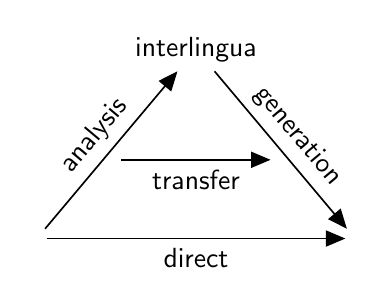
\begin{tikzpicture}[>=triangle 45,font=\sffamily]
    \node (X) at (0,0) {interlingua};
    \node (K) [below left=1cm and 0.05cm of X]  {};
    \node (Y) [below left=2cm and 1cm of X]  {};% 2cm below, 1cm to the left (optional)
    \node (Z) [below right=2cm and 1cm of X] {};
    \node (J) [below right=1cm and 0.05cm of X] {};
    \draw [semithick,<-] (X) -- (Y) node [midway,above,sloped] {analysis} ;
    \draw [semithick,->] (X) -- (Z) node [midway,above,sloped] {generation} ;
    \draw [semithick,->] (Y) -- (Z) node [midway,below,sloped] {direct};
    \draw [semithick,->] (K) -- (J) node [midway,below,sloped] {transfer}  ;

\end{tikzpicture}
\end{center}
\caption{The Vauquois triangle which illustrates the amount of transfer needed for different levels of intermediate representation.}
\label{fig:vauquois}
\end{figure}

In machine translation, an intermediate representation is an abstraction away from the surface forms of the language. Figure~\ref{fig:vauquois} shows the Vauquois triangle, a common illustration of different levels of intermediate representation. 

At the bottom of the triangle, there is no intermediate representation and translation is performed on a word-for-word basis. At the apex of the triangle is interlingual translation, where the source language is first mapped to a language-independent semantic representation, and this representation is then used to generate the target language.

In the middle is (morpho-)syntactic transfer. Here the source language is analysed to a language-dependent intermediate representation (usually based on a combination of syntactic structure and morphosyntactic features) and then transfer rules are applied to convert the source language intermediate representation to one compatible with the target-language generation component. 

\section{Resources}
\label{sec:resources}

In this paper we make use of five sets of linguistic data for five different Uralic languages: Finnish, North Sámi, Erzya, Estonian and Hungarian.
We take the North Sámi and Erzya data from the Giellatekno language technology repository.\footnote{\url{http://giellatekno.uit.no}}
The North Sámi data has primarily been developed by the Divvun and Giellatekno groups at UiT Norgga árktalaš universitehta and the Erzya data has been developed by Jack Rueter at Helsingin yliopisto~\cite{rueter2010adnominal}.
For the Estonian data, we use the \emph{plamk} analyser\footnote{\url{https://github.com/jjpp/plamk}} written by Jaak Pruulmann-Vengerfeldt, for Finnish, \emph{omorfi}~\cite{pirinen2015omorfi}\footnote{\url{https://github.com/flammie/omorfi}}  and for Hungarian, hunmorph~\cite{tron2005hunmorph}.\footnote{\url{http://mokk.bme.hu/resources/hunmorph/}}

% GT: sme, myv
% Omorfi
% plamk




\section{Strategies}

There a different ways to fix systematic mismatches.
We evaluate the followings:

\subsection{Relabelling}

An obvious approach to getting around the problem of divergent tagsets is to simply perform relabelling. This is where you replace the canonical tags in one language with their equivalents in the other language, or with a common equivalent in both languages. 

\begin{center}
\begin{tabular}{c}
+CC $\rightarrow$ \textless{}cnjcoo\textgreater{} $\leftarrow$ +J+Coord
\end{tabular}
\end{center}

However, this solution has its disadvantages. 
Even though +J and +CC both are used for conjuctions, the \emph{plamk} tag is also used with subordinating and other  conjunctions, while the Giellatekno tag excludes those. Relabelling +J+Coord to +CC and any other +J to +CS might work on the analyser, but will not work in a disambiguation rule saying ``select the noun reading if the word to the right is tagged +J'', here we need to relabel +J to (+CS or +CC). In the opposite direction, +CS would need to be relabelled to (+J but not +Coord). The distinction between these may be irrelevant for the translation process (in all cases, \emph{ja} in North Sámi will be translated to \emph{ja} in Estonian), but for the intervening grammatical tools, it may be vital to make (or not) the distinction.

\subsection{Interlingua}

Another potential solution is to use a semantic interlingua (see description in section~\ref{sec:interrep}). This is the approach adopted by the machine translation system based on Grammatical Framework~\cite{ranta2011grammatical}.\footnote{\url{http://grammaticalframework.org}} In this framework there is no direct transfer of morphological features.

\section{Specific linguistic issues}

There are a number of linguistic issues in RBMT.
We cover the following in detail:

\subsection{Copula}

There are two main copula constructions in the Uralic languages, the first functions more or less like in the Germanic languages. The copula is a normal verb that agrees with the subject. The second copula construction works like in the Turkic languages. In languages with the Turkic-style copula, it does not typically surface in the third-person singular present tense. In our examples, North Sámi, Finnish and Estonian are of the Germanic type, while Hungarian and Erzya are of the Turkic type.

\begin{center}
\begin{scriptsize}
\begin{tabular}{lll}
   & `She is a student.' & `She was a student.' \\
North Sámi & Son lea studeanta. & Son lei studeanta. \\
Erzya & Сон студент. & Сон студентель.  \\
Finnish & Hän on opiskelija. & Hän oli opiskelija. \\
Estonian & Ta on üliõpilane. & Ta oli üliõpilane. \\
Hungarian & Ő hallgató. & Ő hallgató volt. \\
\end{tabular}
\end{scriptsize}
\end{center}

In North Sámi, Finnish and Estonian, the treatment of \emph{lea, on} is similar. It is a verb which inflects and agrees like other verbs.

There are divergences when we look at the Erzya and Hungarian examples. Although they have the same structure, zero copula in the present tense and surfaced copula in the past tense. The morphological analyser for Erzya treats the copula as a derivation:

  студент+N+Sg+Nom+Indef+Der/Pr+V+Ind+Prs+ScSg3
  
Where in Hungarian it is simply omitted in the present (if it surfaced it would be \emph{van}), and in the past it is considered a verb form.

\subsection{Non-finite verb forms}

Non-finite verb forms are infinitives and participles on the on hand and derivations on the another. There are a different number of them between languages and their tasks vary from being syntactic arguments of constructions to derived words, and a wide range of analyses are used to accommodate that. There are some differences in the table~\ref{table:non-finite}

\begin{table}
\centering
\begin{scriptsize}

\begin{tabular}{lll}
\textbf{Language} & \textbf{Sentence} & \textbf{Non-finite tag} \\
\hline
           &  `I see the man who is running' & \\
North Sámi & Oidnen dievddu viehkame & Actio+Ess \\
Erzya & Неян цёранть, конась чийни. & Der/Ы+ActPrcShort+A \\
Finnish & Näen miehen juoksemassa. & InfMA+Ine\\
Estonian & Näen meest, kes jookseb. & --- \\
Hungarian & Látom a futó embert. & /VERB[IMPERF\_PART]/ADJ \\
\hline
           &  `While running I saw the man' & \\
North Sámi & Oidnen dievddu viegadettiinan. & Ger+Px1Sg\\
Erzya & Неян чийниця цёранть. & Der/Ыця+ActDemPrc+A \\
Finnish & Näin miehen juostessani. & InfE+Ine+PxSg1 \\
Estonian & Jooksmise ajal nägin ma meest. &  Der/mine+Gen \\
Hungarian & Futás közben láttam az embert.& /VERB[GERUND]/NOUN \\
\hline
           &  `I see the running man.' & \\
North Sámi &  Oainnán viehkki dievddu. & PrsPrc \\
Erzya & Чийнемась седень кецявты. & Der/ОмА+Nom\\
Finnish & Näen juoksevan miehen.  & PrsPrc  \\
Estonian & Näen jooksvat meest. & Der/v+A+Nom\\
Hungarian & Látom a futó embert. & /VERB[IMPERF\_PART]/ADJ \\
\hline
           &  `Running is fun.' & \\
North Sámi & Viehkan lea suohtas.  & Actio+Nom \\
Erzya & Мелезэнь тукшны чийнемась. & Der/ОмА+Nom\\
Finnish & Juokseminen on kivaa.  &  Der/minen+Nom \\
Estonian & Jooksmine on lahe. & Der/mine+Nom \\
Hungarian & A futás jó dolog.& /VERB[GERUND]/NOUN \\
\hline
           &  `I like running.' & \\
North Sámi &   Liikon viehkat. & Inf \\
Erzya & Чийнемстэ неия цёранть. & Inf+Ela \\
Finnish & Pidän juoksemisesta.  & Der/minen+Ela  \\
Estonian & Mulle meeldib joosta. & Inf \\
Hungarian & Szeretem futni.& /VERB<INF> \\
\hline
\end{tabular}
\caption{Examples of the use and tagging of non-finite verb forms in the languages in our sample. It is not to be expected that the tags are completely equivalent, but for example, given the similarity in structure, should there be a difference in annotation between Finnish PrsPrc and Estonian Der/v+A?}
\label{table:non-finite}
\end{scriptsize}

\end{table}


% I see the man who is running.
% While running I saw the man.
% I see the running man.
% Running is fun.
% I like running.

% Näen miehen juoksemassa. & InfMA+ine
% Näin miehen juostessani. & InfE+Ine+PxSg1
% Näen juoksevan miehen.   & PrsPrc
% Juokseminen on kivaa.    & Der/minen
% Pidän juoksemisesta.     & Der/minen+Ela

% Oidnen dievddu viehkame & Actio+Ess
% Oidnen dievddu viegadettiinan & Ger+Px1Sg
% Oainnán viehkki dievddu & PrsPrc
% Viehkan lea suohtas & Actio+Nom
% Liikon viehkat & Inf

% näen meest, kes jookseb.  & [who runs]
% jooksmise ajal nägin ma meest. & Der/mine+N+Sg+Gen
% näen jooksvat meest.     & Der/v+A+Sg+Par
% jooksmine on lahe        & Der/mine+N+Sg+Nom
% mulle meeldib joosta.    & inf


% I see the man who is running.
% Látom a futó embert.
% While running I saw the man.
% Futás közben, láttam az embert.
% I see the running man.
% Látom a futó embert.
% Running is fun.
%A futás jó dolog.
% I like running.
%Szeretem a futást.

\subsection{Derivation, compounding and lexicalisation}

A classical problem in computational morphologies lies in question of lexicalisation and productivity of certain processes; is a morphologically created word-form a new word or a form of a, possibly distant root.
Morphologies take widely different and opposing approaches to this ranging from lexicalise-everything to collect-everything. See examples below:
\begin{center}
\begin{scriptsize}
\begin{tabular}{lllll}

   & `to drink' & `a drink' & `drinker' & `brewery' \\
North Sámi & juhkat & juhkamuš & --- & vuolla·buvttadeaddji \\
Erzya & симемс & симема-пель  & симиця & пиянь завод \\
Finnish & juoda & juo-ma & juo|ja &  olut·tehdas\\
Estonian & jooma &joo|gi  & joo| &  õlle·tehas\\
Hungarian & iszik & ital & iv|ó & sör·főzde  \\
\end{tabular}
\end{scriptsize}
\end{center}

The symbols `·', `-' and `|' stand for compounding, inflection and derivation, respectively.

\subsection{Pronouns and determiners}

The distinction between pronoun and determiner is not widely made in traditional grammars of most Uralic languages. Words which may be considered both pronouns and determiners are lumped into a single morphosyntactic class (usually pronoun). Consider the following examples involving the word `this'

\begin{center}
\begin{scriptsize}
\begin{tabular}{lll}
  & `I see this house.' & `I see this.' \\
  North Sámi & Oainnán dán viesu. & Oainnán dán. \\
  Erzya & Неян те_{\textsc{det}} кудонть. & Неян тень_{\textsc{pron}}. \\
  Finnish & Mä näen tämän_{\textsc{pron}} talon. & Mä näen tämän_{\textsc{pron}}. \\
  Estonian & Ma näen selle_{\textsc{pron}} maja. & Ma näen selle_{\textsc{pron}}. \\
  Hungarian & Nézem ezt_{\textsc{det/noun}} a_{\textsc{art}} házat. & Nézem azt_{\textsc{det/noun}}  \\
\end{tabular}
\end{scriptsize}
\end{center}
   
In traditional grammars of North Sámi, Finnish and Estonian both the pronominal and the modifier analyses of `this' are classified as pronouns. In Hungarian and Erzya, a distinction is made, with Hungarian making a pronoun/determiner distinction and Erzya making a distinction between quantifier (determiner) and nominalised quantifier.

If we consider a standard definition of \emph{pronoun} to be `that which stands in place (pro-) of a noun phrase (-noun)' then we can see that in the above, only the tools for Erzya follow this. The other languages leave the distinction to tools later in the pipeline. 

% Эрьва кудонть неян.
% неян эрьванть 
% эрьва+Qnt+Der/MWN+N+Sg+Gen+Def

\subsection{Non-inflecting words}
% conj, adv, adpos

All languages in the Uralic family have a wide variety of non-inflecting word forms. Depending on the grammatical tradition followed by the language resource these may be simply lumped into a single class, or they may have extensive syntactic or semantic subcategorisation. Table~\ref{table:noninflect} gives a number of examples of non-inflecting words and the equivalent morphological analyses they receive in each of the languages we are studying. To a machine translation practitioner, these distinctions are largely superfluous, \emph{ja} in North Sámi will be translated as \emph{ja} in Finnish and \emph{ja} in Estonian. However, the distinctions may be vital for the intervening disambiguation tools, and as such need to be taken into account.


\begin{table}
\centering
\begin{scriptsize}
  \begin{tabular}{lccccc}
      & \textbf{North Sámi} & \textbf{Erzya} & \textbf{Finnish} & \textbf{Estonian} & \textbf{Hungarian} \\
     and & ja+CC & марто+Po+COM & ja Part & ja+J & és /CONJ \\
     very & hui+Adv & пек+Adv+AdA & tosi Part & väga+Adv & nagyon /ADV \\
     under & vuolde+Po & алов+Po+Lat & alle Part & alla+K & alatt /POSTP \\
     now & dál+Adv & ней+Adv+Temp & nyt Part & praegu+Adv & most /ADV \\
     hello & bures+Interj & шумбрачи+Interj+Formulaic & moi Part & tere+I & szia /UTT-INT \\
  \end{tabular}
\end{scriptsize}  
  \caption{Some examples of non-inflecting words with divergent morphological and syntactic annotation. In terms of morphology, the transfer of these tags may be a simple one-to-one substitution. However the syntactic environments may vary substantially.}
   \label{table:noninflect}
\end{table}


\section{Guidelines}
\label{sec:guidelines}

\subsection{Separation of lexicon and morphotactics}

One of the main components of any rule-based system for morphologically-complex languages is a lexicon consisting of stems and inflectional/derivation categories. In some cases, such as for Finnish, these are partly provided by a state institution, such as a language board. In other cases they are the product of many years of work.

Although categorising stems for inclusion in a morphological lexicon (many contain over 100,000 entries) can take a substantial amount of work, even if done semi-automatically, implementing the morphotactics (that is, the rules covering inflection, derivation and compounding) may take substantially less time.

\subsection{Maximise parallelism}

In line with the Universal Dependencies project (see~\ref{sec:universal}), we propose the adoption of a principle of maximum parallelism. In short ``things that are the same should be tagged the same''. We do not propose that this should mean that all distinctions should be made in all languages. For example, those Uralic languages without object conjugation should not be required to adopt the agreement tags of those that have it. But it should be possible to come up with principled and consistent guidelines for closed categories.

%\subsection{Adoption of maximal differences}
% prn vs. det
% lumping is easier than splitting

\section{Universal dependencies}
\label{sec:universal}

Universal dependencies is a large multi-language project~\cite{mcdonald2013universal} aiming at common tagset for part-of-speech, morphosyntactic features and dependency relations.
We do not propose adopting the exact tagset of the universal dependency project. Most projects working on Uralic languages have been ongoing for many years and the tools that they create are used for more than just machine translation. What we find more important is to adopt, or make available tools based on a consistent theoretical background and consistent morphosyntactic description. This could form the basis of a kind of \emph{universal} morphosyntactic interlingua for the Uralic languages. These tools do not have to replace the current tools, and may be automatically generated from them, but they must be consistent. A systematic mapping needs to be considered while developing.
The national Uralic languages have specifications for universal dependencies~\cite{ud-finnish,ud-estonian,ud-hungarian}. But these specifications differ in unnecessary ways. For example, consider the annotation of `that house' in the two treebanks for Finnish: Turku Dependency Treebank (TDT) and FinnTreeBank (FTB); and Hungarian:

\begin{center}
\begin{scriptsize}
\begin{tabular}{llll}
            & \multicolumn{2}{l}{this} & house \\
  Finnish (TDT)   & \multicolumn{2}{l}{tämä_{\textsc{PRON}}} & talo_{\textsc{NOUN}} \\
  Finnish (FTB)  & \multicolumn{2}{l}{tämä_{\textsc{DET}}} & talo_{\textsc{NOUN}} \\
  Hungarian & az_{\textsc{PRON}} & a_{\textsc{ART}} & ház_{\textsc{NOUN}} \\
\end{tabular}
\end{scriptsize}
\end{center}


% examples of non-equivalent things

\section{Concluding remarks}
\label{sec:conclusion}

%We have shown obstacles for RBMT of Uralic languages.
%We have developed a system that works.
%We have good guidelines developed over 10 years of experience.
%In future it would be interesting to have more systems that work.

Rule-based machine translation provides a fascinating basis for exploring real linguistic differences between the Uralic languages. However, as we have shown, in current state-of-the-art tools, real linguistic differences are hidden behind a combination of incompatible tagsets and idiosyncratic traditional grammatical norms. We do not propose that the North Sámi adopt the Finnish norms or the Hungarians the Erzya norms, instead we propose developing a common morphological annotation scheme for the Uralic languages based on guidelines of the Universal dependencies project. It is not our aim for this to supercede national standards, but provide a common bridge between them to facilitate the cross-linguistic study and functional rule-based machine translation.

\section*{Acknowledgements}
Heiki-Jaan Kaalep, Jack Rueter, László Tihany as well as the anonymous reviewers have all contributed to the language examples, the remaining mistakes are ours.

\appendix

\section{Example of Universal dependencies for Uralic languages}

Example is shown in table~\ref{table:wetdream}.

\begin{table}
\begin{scriptsize}

\hrule
  \begin{tabular}{llll}
     \emph{James}  & \emph{ja} & \emph{Mary} &  \\
     PROPN &  CONJ & PROPN &   \\ 
     Number=Sing|Case=Nom &   & Number=Sing|Case=Nom &   \\ 
     \emph{leaba} & \emph{gárdimis} & \emph{.}    & \\
     VERB &  NOUN & PUNCT  & \\
          Mood=Ind|Tense=Pres|Person=3|Number=Dual &  Number=Sing|Case=Loc &   & \\

  \end{tabular}\\
\hrule
  \begin{tabular}{llll}
     \emph{Джеймс} & \emph{марто} & & \\
     PROPN & CONJ &  & \\
     Number=Sing|Case=Nom|Definite=Ind &  &   \\
     \emph{Марит} & \emph{садпиресэ-}  & & \\
     PROPN & NOUN & & \\
     Number=Plur|Case=Nom|Definite=Ind & Case=Ine|Definite=Ind & & \\
      \emph{-ть} & . & &\\
       VERB & PUNCT &  & \\
  Mood=Ind|Tense=Pres|Pers[subj]=3|Number[subj]=Plur & \\

  \end{tabular}\\
\hrule
  \begin{tabular}{llll}
  \emph{James} & \emph{ja} & \emph{Mary} & \\
     PROPN    &  CONJ     & PROPN &   \\ 
     Number=Sing|Case=Nom &   & Number=Sing|Case=Nom   \\ 
  \emph{ovat} & \emph{puutarhassa} & \emph{.} &  \\
  VERB & NOUN & PUNCT &  \\
  Mood=Ind|Tense=Pres|Person=3|Number=Plur & Number=Sing|Case=Ine &  & \\
  \end{tabular}\\
\hrule
  \begin{tabular}{llll}
  \emph{James} & \emph{ja} & \emph{Mary} & \\
     PROPN    &  CONJ     & PROPN &   \\ 
     Number=Sing|Case=Nom &   & Number=Sing|Case=Nom   \\ 
   \emph{on} & \emph{aias} & \emph{.} & \\
   VERB & NOUN & PUNCT & \\
  Mood=Ind|Tense=Pres|Person=3|Number=Plur & Number=Sing|Case=Ine &  & \\
  \end{tabular}\\
\hrule
  \begin{tabular}{llll}
   \emph{James} & \emph{és} & \emph{Mary} & \\
    PROPN    &  CONJ     & PROPN &   \\ 
     Number=Sing|Case=Nom &   & Number=Sing|Case=Nom   \\ 
   \emph{kértben} & \emph{.} & & \\
   NOUN & PUNCT & & \\
   Number=Sing|Case=Ine &  & & 

  \end{tabular}
  \hrule
  \caption{An example of applying universal part-of-speech tags and morphological features to the Uralic languages. Note how the massive differences in annotation are reduced to only the linguistically relevant compared to Table~\ref{table:albtraum}.}
  \label{table:wetdream}
  \end{scriptsize}
\end{table}

\bibliographystyle{unsrt}
\bibliography{iwclul2016}

\end{document}
